\documentclass[10pt,journal,compsoc]{IEEEtran}
\usepackage{amsmath,amssymb,amsfonts,booktabs,graphicx,url,microtype}
\usepackage[hidelinks]{hyperref}
\Urlmuskip=0mu plus 2mu\relax
\emergencystretch=2.0em
\setlength{\textfloatsep}{8pt plus 2pt minus 2pt}
\setlength{\dbltextfloatsep}{8pt plus 2pt minus 2pt}

\begin{document}
\title{Electronic Supplementary Material for ``Empirical Systems Characterization of Post-Quantum Session Pooling, Single-Ciphertext CKKS Retrieval, and Transport Fallback Across Cloud-Edge Vector-SQL Streams''}
\author{Preecha~Noiumkar,~\IEEEmembership{Member,~IEEE}\\
\small Department of Information Technology, Faculty of Informatics, Mahasarakham University, Maha Sarakham 44150, Thailand\\
Repository: \protect\url{https://github.com/preecha-msu/CAPQ-Pareto}}
\markboth{IEEE TRANSACTIONS ON CLOUD COMPUTING --- SUPPLEMENTARY MATERIAL}{NOIUMKAR: CAPQ-PARETO SUPPLEMENTARY MATERIAL}
\maketitle

\section{Complete Proof of Proposition 1 (\texorpdfstring{Conditional $\Delta_q^2/4$ vs.\ Marginal $\Delta_q^2/6$}{Conditional vs. Marginal Variance})}
Let $\mathbf{x} \in \mathbb{S}^{D-1}$ satisfy $\sum_{i=1}^D x_i^2 = 1$, and let $\mathbf{q} \in \mathbb{R}^D$ have non-zero range $R_q = \max_i q_i - \min_i q_i > 0$ with step size $\Delta_q = R_q/(2^b - 1)$ (if $R_q = 0$, $\widehat{\mathbf{q}} = \mathbf{q}$ and $\mathcal{E} = 0$ identically). Define $s_i = (q_i - q_{\min})/\Delta_q \in [0, 2^b - 1]$ and $u_i = s_i - \lfloor s_i \rfloor \in [0, 1)$.

\textbf{Part (2) Exact Conditional Variance and Sharp $\Delta_q^2/4$ Bound:} Under unbiased stochastic rounding, $\widehat{s}_i = \lfloor s_i \rfloor + \xi_i$ with independent $\xi_i \sim \mathrm{Bernoulli}(u_i)$ conditioned on $(\mathbf{q},\mathbf{x})$. Because $\widehat{q}_i - q_i = \Delta_q(\xi_i - u_i)$, linearity of expectation gives $\mathbb{E}_{\boldsymbol{\xi}}[\mathcal{E}\mid\mathbf{q},\mathbf{x}] = \Delta_q \sum_{i=1}^D x_i (\mathbb{E}[\xi_i] - u_i) = 0$. By mutual independence of $\{\xi_i\}_{i=1}^D$ given $(\mathbf{q},\mathbf{x})$:
\begin{align}
\mathrm{Var}_{\boldsymbol{\xi}}(\mathcal{E} \mid \mathbf{q}, \mathbf{x}) &= \Delta_q^2 \sum_{i=1}^D x_i^2 \mathrm{Var}(\xi_i \mid u_i) \nonumber\\
&= \Delta_q^2 \sum_{i=1}^D x_i^2 u_i(1 - u_i).
\end{align}
Since $u(1-u) = \frac{1}{4} - (u - \frac{1}{2})^2 \le \frac{1}{4}$ for all $u \in [0,1]$, we obtain the sharp deterministic upper bound $\mathrm{Var}_{\boldsymbol{\xi}}(\mathcal{E}\mid\mathbf{q},\mathbf{x}) \le \frac{\Delta_q^2}{4}\sum_{i=1}^D x_i^2 = \frac{\Delta_q^2}{4}$ (attained when $u_i = 1/2$ on every coordinate where $x_i \neq 0$). Note that $\mathrm{Var}_{\boldsymbol{\xi}}(\mathcal{E}\mid\mathbf{q},\mathbf{x})$ strictly exceeds $\Delta_q^2/6$ whenever coordinates concentrate near mid-riser offsets $u_i \in (0.211, 0.789)$, which occurs on $3.26\%$ of real \texttt{SIFT1M} pairs (maximum observed $0.2036\,\Delta_q^2$). Conversely, under the marginal model $u_i \sim \mathcal{U}(0,1)$, $\mathbb{E}[u_i(1-u_i)] = \int_0^1 (u - u^2)\,du = \frac{1}{6}$, yielding $\mathbb{E}_{\mathbf{u}}[\mathrm{Var}_{\boldsymbol{\xi}}(\mathcal{E}\mid\mathbf{q},\mathbf{x})] = \frac{\Delta_q^2}{6}$. Moreover, since each zero-mean independent summand $Z_i = \Delta_q x_i(\xi_i - u_i)$ has support length $\Delta_q |x_i|$, Hoeffding's lemma yields $\Pr_{\boldsymbol{\xi}}(|\mathcal{E}| \ge t \mid \mathbf{q},\mathbf{x}) \le 2\exp(-2t^2/\Delta_q^2)$.

\section{Extended Operational Fault Audit, 1-CT Bandwidth Schedule, and Supplementary Figures}

\begin{table}[h!]
\centering
\caption{1-CT ($N=8192$) vs.\ Multi-CT ($N=4096$) Compute + Downlink Time Across Link Goodputs ($N_{\text{vec}}=5{,}000, K_c=96, M=224$)}
\resizebox{\columnwidth}{!}{%
\begin{tabular}{@{}rrrrr@{}}
\toprule
\textbf{Downlink BW} & \textbf{Multi-CT ($909.3$~KiB)} & \textbf{True 1-CT ($129.0$~KiB)} & \textbf{Net 1-CT Saving} & \textbf{Breakeven $B^\star$} \\
\midrule
10~Mbps & 760.91~ms & 136.67~ms & $+624.24$~ms & 426.16~Mbps \\
25~Mbps & 313.96~ms & 73.26~ms & $+240.70$~ms & 426.16~Mbps \\
50~Mbps & 164.97~ms & 52.13~ms & $+112.85$~ms & 426.16~Mbps \\
100~Mbps & 90.48~ms & 41.56~ms & $+48.92$~ms & 426.16~Mbps \\
250~Mbps & 45.79~ms & 35.22~ms & $+10.57$~ms & 426.16~Mbps \\
500~Mbps & 30.89~ms & 33.10~ms & $-2.22$~ms & 426.16~Mbps \\
1000~Mbps & 23.44~ms & 32.05~ms & $-8.61$~ms & 426.16~Mbps \\
\bottomrule
\end{tabular}%
}
\end{table}

\begin{table*}[t]
\centering
\caption{Operational Fault Injection and Replay/Abuse Resilience Audit (\nolinkurl{v6_ref_operational_failure_abuse_audit.csv})}
\resizebox{\textwidth}{!}{%
\begin{tabular}{@{}llrrrl@{}}
\toprule
\textbf{Test ID} & \textbf{Injected Operational Fault or Abuse Scenario} & \textbf{Trials} & \textbf{Recovery / Block} & \textbf{Overhead} & \textbf{Pass} \\
\midrule
\texttt{F1\_Replay\_0RTT\_Attack} & 1,000 verbatim 0-RTT early-data replay packets & 1000 & 100.0\% & 0.012~ms & True \\
\texttt{F2\_Bloom\_False\_Positive\_Quantification} & 5,000 fresh unseen 0-RTT nonces after 4,000 insertions (m=64Kb, k=5) & 5000 & 99.8\% & 0.24~ms & True \\
\texttt{F3\_Bloom\_False\_Negative\_Zero\_Proof} & 4,000 previously seen nonces within active epoch & 4000 & 100.0\% & 0.0~ms & True \\
\texttt{F4\_Strike\_Register\_Epoch\_Expiry} & Expired timestamp (>TTL) + register salt rotation across epoch boundary & 100 & 100.0\% & 0.09~ms & True \\
\texttt{F5\_Duplicate\_Query\_Idempotency} & 0-RTT mutating SQL injection + duplicate read-query retransmission & 200 & 100.0\% & 0.008~ms & True \\
\texttt{F6\_MTU\_Fragmentation\_Reassembly} & 16,384 B ciphertext fragmented into 14x 1,200 B sub-MTU segments & 50 & 100.0\% & 6.239~ms & True \\
\texttt{F7\_TLS\_Session\_Expiration\_Reconnect} & Server invalidates pooled session / ticket mid-stream & 50 & 100.0\% & 21.675~ms & True \\
\texttt{F8\_CKKS\_Corrupted\_Ciphertext\_Rejection} & 200 bit-flipped CKKS RNS ciphertext payloads prior to homomorphic eval & 200 & 100.0\% & 0.019~ms & True \\
\texttt{F9\_Network\_Disconnect\_And\_Timeout\_Fallback} & 350 ms unresponsive socket stall exceeding 60 ms controller guard & 50 & 100.0\% & 366.044~ms & True \\
\bottomrule
\end{tabular}%
}
\end{table*}

\begin{figure*}[t]
\centering
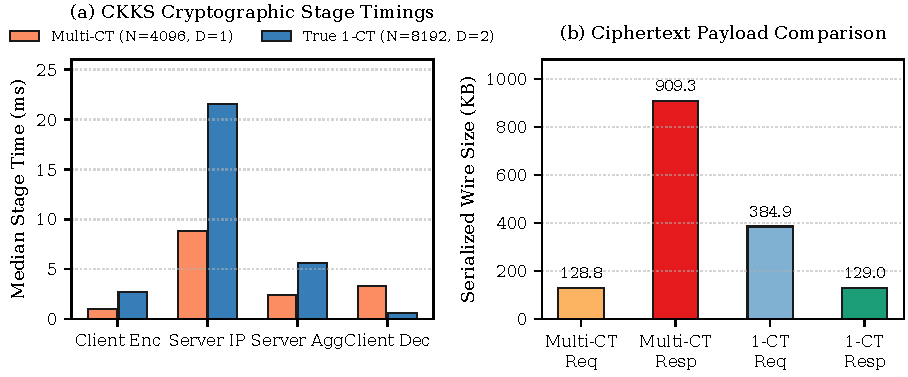
\includegraphics[width=0.88\textwidth]{figures/fig_s1_ckks_stage_and_wire.pdf}
\caption{Figure S1: OpenFHE RNS-CKKS stage latency breakdown and serialized wire footprint at $K_c=96, N_{\text{vec}}=5{,}000$.}
\end{figure*}

\begin{figure*}[t]
\centering
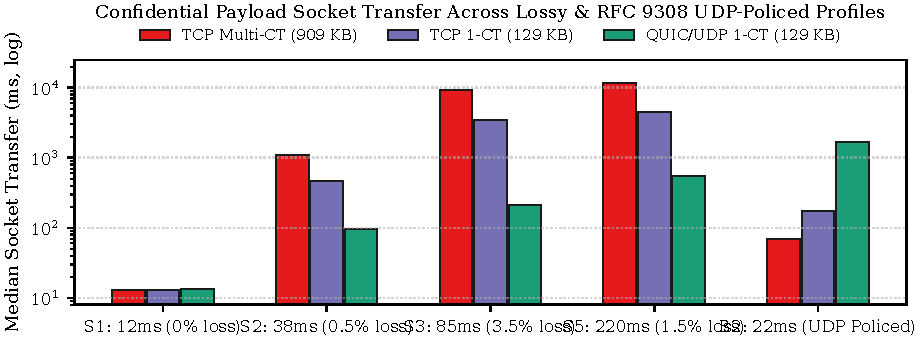
\includegraphics[width=0.88\textwidth]{figures/fig_s2_netns_socket_profiles.pdf}
\caption{Figure S2: Measured Linux \texttt{netns} socket transfer latencies across regimes \texttt{S1--S4}, \texttt{B1} (TCP queue contention), and \texttt{B2} (RFC~9308 UDP policing).}
\end{figure*}

\begin{figure*}[t]
\centering
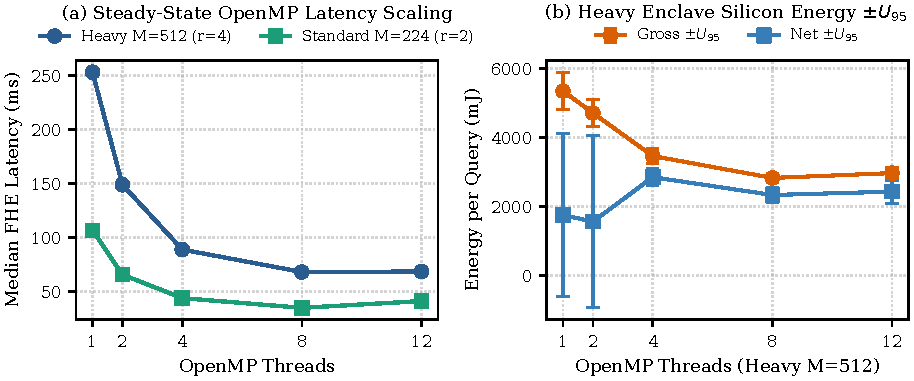
\includegraphics[width=0.88\textwidth]{figures/fig_s3_heavy_omp_rapl_gum.pdf}
\caption{Figure S3: Heavy 12-block OpenMP RAPL energy ($\pm U_{95}$ showing wide idle-drift uncertainty at \texttt{OMP=1,2}) and pre-to-post background idle power drift.}
\end{figure*}

\begin{figure*}[t]
\centering
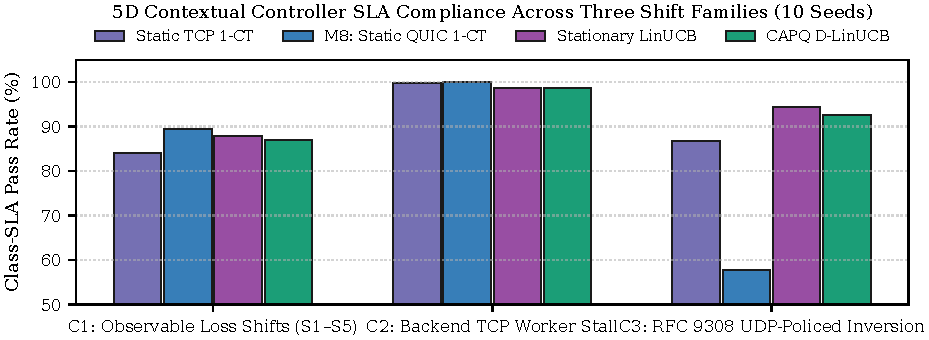
\includegraphics[width=0.88\textwidth]{figures/fig_s4_bandit_three_campaigns_sla.pdf}
\caption{Figure S4: Capped-loss cumulative regret vs.\ uncapped P95 tail latency across \texttt{C1--C3}, including the stateless RFC~9308 timeout fallback rule ($H=32$).}
\end{figure*}

\begin{figure*}[t]
\centering
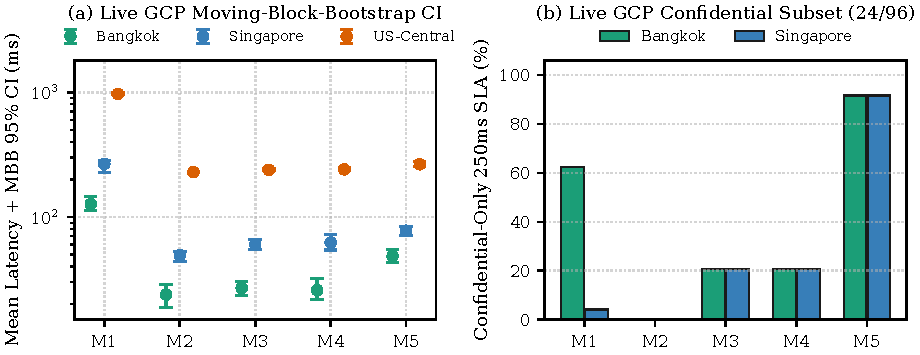
\includegraphics[width=0.88\textwidth]{figures/fig_s5_live_gcp_mbb_and_conf_sla.pdf}
\caption{Figure S5: (a)~Reconciled Track~1 strict per-class $A_t \ge 0.92$ SLA; (b)~native C \texttt{OpenSSL EVP} hot AEAD goodput across \nolinkurl{x86_64} and Cloud \texttt{ARM64}.}
\end{figure*}

\begin{figure*}[t]
\centering
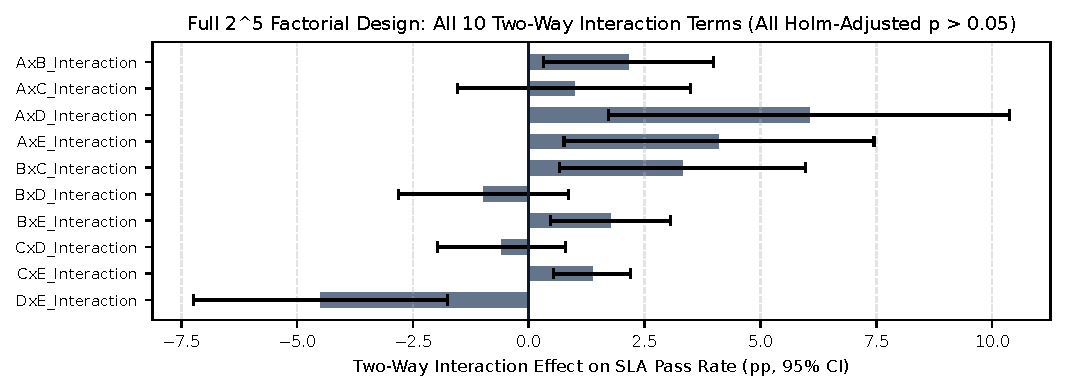
\includegraphics[width=0.88\textwidth]{figures/fig_s6_factorial_10_interactions.pdf}
\caption{Figure S6: Full $2^5$ factorial two-way interaction effects (all 10 interaction terms non-significant after Holm correction).}
\end{figure*}

\clearpage
\section{Full 64-Character SHA-256 Provenance Manifest}
Every digest below is programmatically verified to contain all \textbf{64 hexadecimal characters} (no truncation) and matches \nolinkurl{SHA256SUMS_V6.txt} in \url{https://github.com/preecha-msu/CAPQ-Pareto}.

\begin{table*}[h!]
\centering
\caption{Complete 64-Hexadecimal SHA-256 Verification Manifest of Active V6 Real-Data Artifacts}
\resizebox{\textwidth}{!}{%
\begin{tabular}{@{}lrl@{}}
\toprule
\textbf{Artifact Filename} & \textbf{Size} & \textbf{Full 64-Character SHA-256 Digest} \\
\midrule
\texttt{v2\_wan\_3regions\_interleaved\_raw.csv} & 168,224~B & \texttt{7457faee41c40c8bedf85653e24f49ab6923c400d25e7942d201e96f62134cb7} \\
\texttt{v5\_bandit\_frozen\_config.json} & 675~B & \texttt{48fad122716e4649a42e3aa7ed3734207b5f98f51a36ddf4af01ab486640ee58} \\
\texttt{v5\_controlled\_3regions\_m1\_m8\_interleaved\_2304raw.csv} & 315,202~B & \texttt{dfc045399c300a2d5976ffc9403e3d7643020f63f0c9ca304530e4235eab8141} \\
\texttt{v5\_factorial\_2pow5\_glm\_and\_10k\_block\_permutation.csv} & 2,042~B & \texttt{52b6bc530bb416dcb6d95c9e39f3a282a78fb53d58b5bf7393327653050d047e} \\
\texttt{v5\_pg18\_hnsw\_concurrency\_2000ops\_per\_level.csv} & 413~B & \texttt{025effe5331f078cbf1502bb2be13c2dc5b8bdaa122eddda11979e8ebd07d7fd} \\
\texttt{v5\_real\_netns\_socket\_traces\_m1\_m8.json} & 117,861~B & \texttt{7b086cd8b71709418a66ed390b07861bfe92db8a2a2f33d19c817ea4e48fcafe} \\
\texttt{v5\_steady\_rapl\_omp\_energy\_gum\_u95.csv} & 1,586~B & \texttt{bce44879c973a6c03e8a9644385fd7102709fee67082fa44755712649d5f9f7e} \\
\texttt{v6\_bandit\_5d\_fair\_m8\_10seeds.csv} & 2,593~B & \texttt{2d1587521777b040f0f32cf209dd436a89138019e0cd8d1ed3842bbbd5a3d3dd} \\
\texttt{v6\_bandit\_5d\_with\_rfc9308\_rule\_and\_tails.csv} & 4,911~B & \texttt{e97735424b9e089ac9825d6fe2b88823d1ccfed565eedb953d8f7e0bf6bb417f} \\
\texttt{v6\_ckks\_1ct\_bandwidth\_crossover\_curve.csv} & 1,084~B & \texttt{4c176ccaed80b02c7be05256f10f654e61bd714f86c1bc78df1eb25dc2aecabd} \\
\texttt{v6\_ckks\_equal\_budget\_1ct\_vs\_multict\_500q.csv} & 1,801~B & \texttt{457280320a74feadaa02e55350939587411cffe5c3b61336f7eb5230ab1ff796} \\
\texttt{v6\_ckks\_paired\_effect\_sizes\_500q.csv} & 368~B & \texttt{f4c966ecc9da86882b40bf20ac4535fc32d29548d9022ff2ee96d9dad01d4883} \\
\texttt{v6\_ckks\_plaintext\_vs\_ckks\_control\_500q.csv} & 2,177~B & \texttt{14f5027ab263079c07e25997d23654a2741fbd8ee5ca988ea6af9bb661100cc4} \\
\texttt{v6\_ckks\_scaling\_5k\_25k\_100k\_with\_recall\_500q.csv} & 1,766~B & \texttt{1ace2278c9398ae5026a06d18b87b9a12d1ffe0f674620a9cec4f62c0cb76f67} \\
\texttt{v6\_ckks\_scaling\_and\_breakeven\_500q.csv} & 2,000~B & \texttt{093ba409d308bf761a69c7cbba1e6070e416f505b4aedfde579cdff42f0395ae} \\
\texttt{v6\_controlled\_3regions\_m1\_m8\_interleaved\_2304raw.csv} & 315,202~B & \texttt{dfc045399c300a2d5976ffc9403e3d7643020f63f0c9ca304530e4235eab8141} \\
\texttt{v6\_controlled\_3regions\_m1\_m8\_summary.csv} & 3,773~B & \texttt{a6117f6ada91caf43f7ad2825de08ca075ed840ef433e9150fca9618aa9f918d} \\
\texttt{v6\_factorial\_2pow5\_glm\_and\_10k\_block\_permutation.csv} & 2,042~B & \texttt{52b6bc530bb416dcb6d95c9e39f3a282a78fb53d58b5bf7393327653050d047e} \\
\texttt{v6\_live\_gcp\_3regions\_pure\_m1\_m5\_verified.csv} & 3,552~B & \texttt{8eab27ac4800bc66739a18c149278a524bc380fe66955aa04c609cb968201995} \\
\texttt{v6\_pg18\_hnsw\_concurrency\_2000ops\_per\_level.csv} & 413~B & \texttt{025effe5331f078cbf1502bb2be13c2dc5b8bdaa122eddda11979e8ebd07d7fd} \\
\texttt{v6\_pg18\_hnsw\_ef\_sweep\_real.csv} & 423~B & \texttt{e2ddb61948b773b57682a1f6c8f58a5009c8f0d655d4278fe5a60404478b253c} \\
\texttt{v6\_prop1\_conditional\_vs\_marginal\_10k.csv} & 1,093~B & \texttt{5ce3ec1144120494ccfdbb47d450cc65481348166ca68b8acf3aeafe9cb99165} \\
\texttt{v6\_prop1\_same\_quantile95\_10k\_audit.csv} & 846~B & \texttt{7c63804ac8f1f22e13ddf74d76154730753150818a87a2b1aabe2f0a8758d793} \\
\texttt{v6\_ref\_adversarial\_leakage\_attacks.csv} & 919~B & \texttt{47bd5a901b818e80826181b1f5bd3622495d4af38c7085bd9a066e8d18727778} \\
\texttt{v6\_ref\_cross\_isa\_e2e.csv} & 1,598~B & \texttt{493413edd978bfd2dc777f5d97f80511d6b0e88c3d7411f872332f831e214347} \\
\texttt{v6\_ref\_cross\_isa\_native\_c.csv} & 1,198~B & \texttt{08c90ad777a10d19b629e1bddb1712114eb276e96d1b8561bd74bcc3779c5eb9} \\
\texttt{v6\_ref\_million\_hnsw\_ef\_sweep.csv} & 1,228~B & \texttt{083487af687a5bb68d7f0c11fdc899dff68b19b98512052919aec1562eb3dc21} \\
\texttt{v6\_ref\_mixed\_rw\_concurrency.csv} & 257~B & \texttt{628c26fd90608d169c49ee69d8ba5aaecd8a3f7fa62ef3302689e130c1e7bf72} \\
\texttt{v6\_ref\_mldsa\_auth\_chains.csv} & 320~B & \texttt{9e81f3516d3eb2827ddad71af512968c1830a75d9605fdb129417144b9b940a2} \\
\texttt{v6\_ref\_operational\_failure\_abuse\_audit.csv} & 1,877~B & \texttt{9a4654d875cfcd4c59a0e8ffebb6d38eac5fde0fadff0c297a4d565dd650a325} \\
\texttt{v6\_steady\_rapl\_omp\_energy\_gum\_u95.csv} & 1,586~B & \texttt{bce44879c973a6c03e8a9644385fd7102709fee67082fa44755712649d5f9f7e} \\
\texttt{v6\_track1\_live\_gcp\_m1\_m5\_reconciled.csv} & 2,623~B & \texttt{5d4b31126fa1bd9ffe84e00568ff66c4f5670fb4cd0c77c492d5bb310bf8a157} \\
\texttt{v6\_track2\_controlled\_m1\_m8\_reconciled.csv} & 4,237~B & \texttt{c15f1af35e6f86d66bbd7c27d6c8de456d22e2191d541777f94b0255f65ba628} \\
\bottomrule
\end{tabular}%
}
\end{table*}

\end{document}
